\chapter{IDEF0-диаграмма алгоритма работы программы}
\label{cha:appendix1}

\begin{figure}[h]
	\centering
	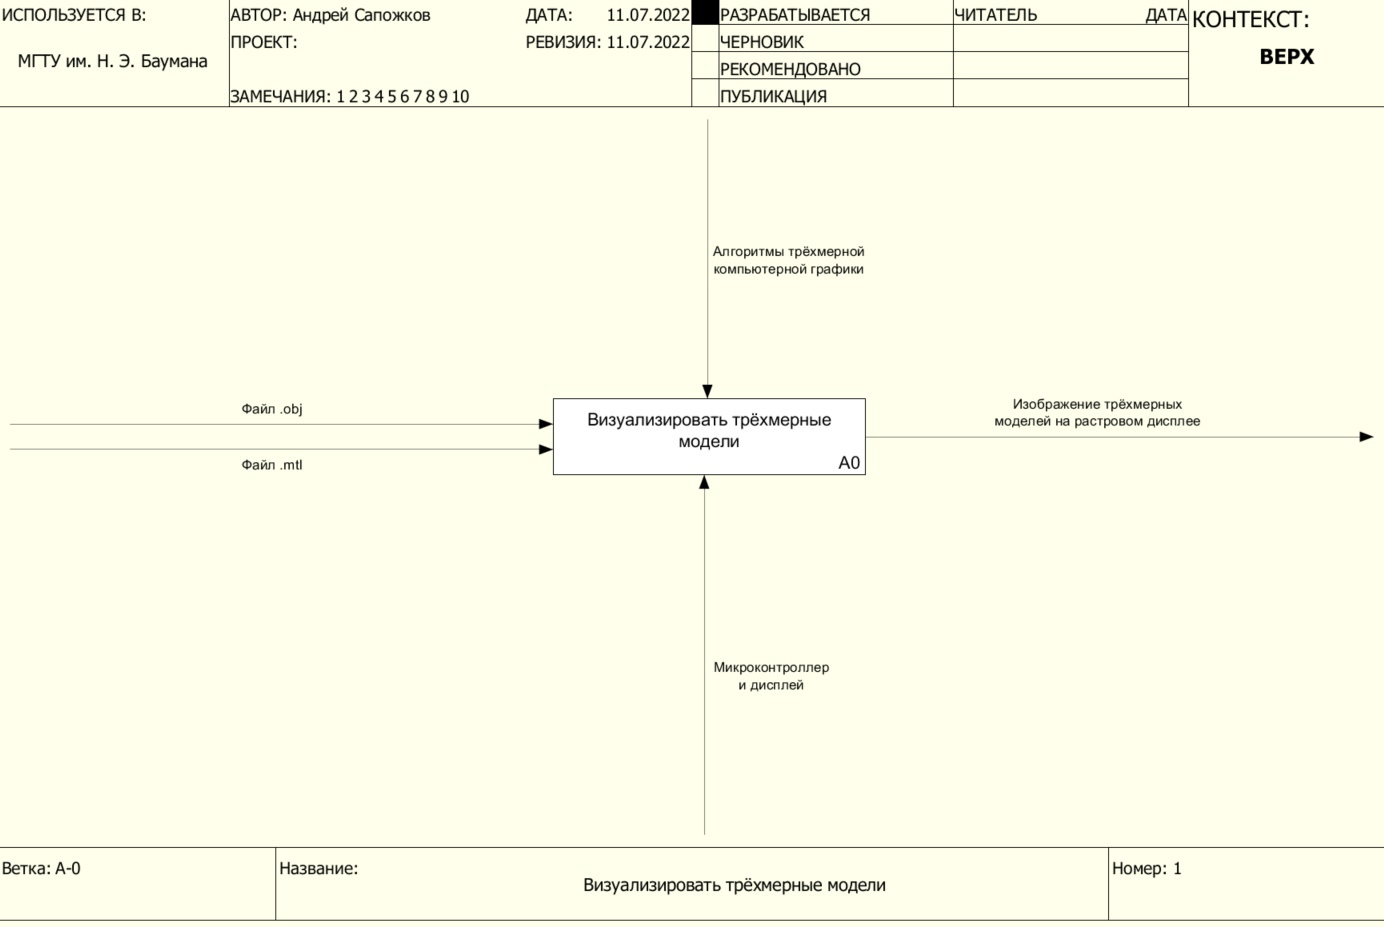
\includegraphics[width=\textwidth ]{img/IDEF0/A0.jpg}
	\caption{Верхний уровень диаграммы.}
\end{figure} 

\begin{figure}[h]
	\centering
	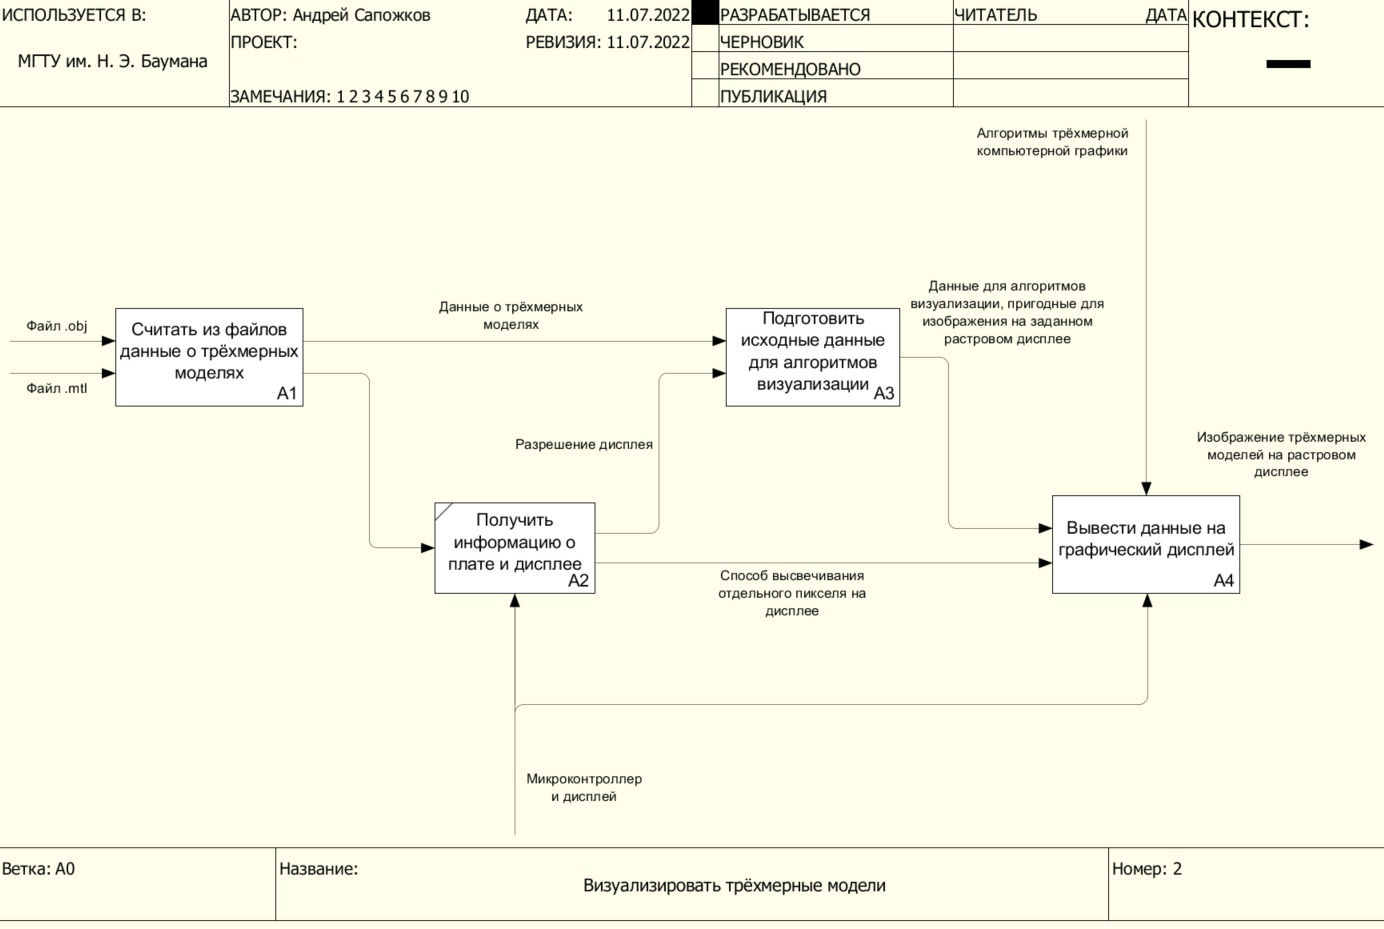
\includegraphics[width=\textwidth ]{img/IDEF0/A0_decomposition.jpg}
	\caption{Декомпозиция уровня A0.}
\end{figure} 

\begin{figure}[h]
	\centering
	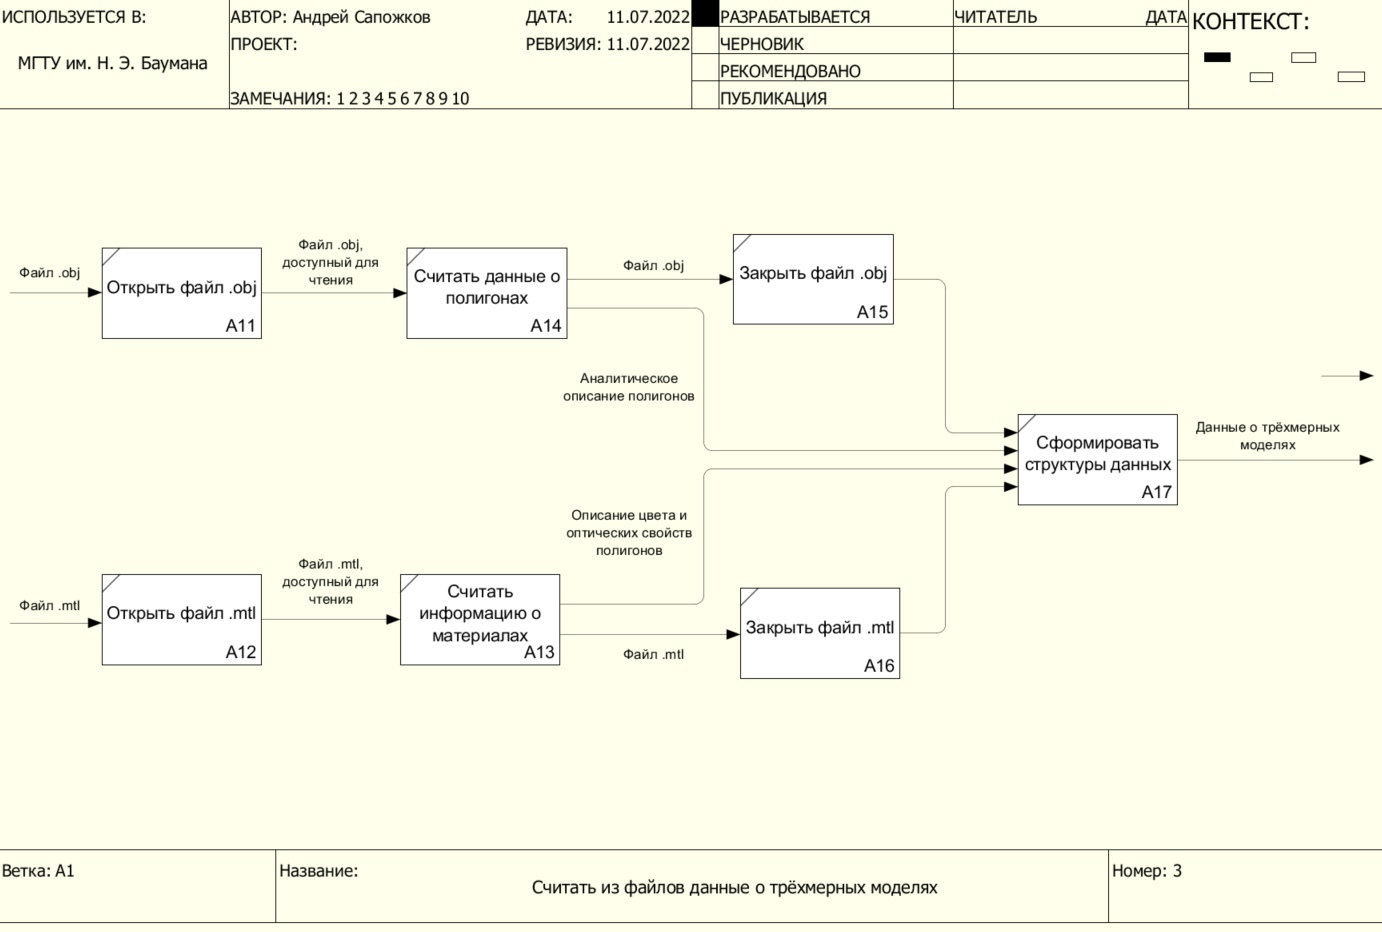
\includegraphics[width=\textwidth ]{img/IDEF0/A1_decomposition.jpg}
	\caption{Декомпозиция уровня A1.}
\end{figure} 

\begin{figure}[h]
	\centering
	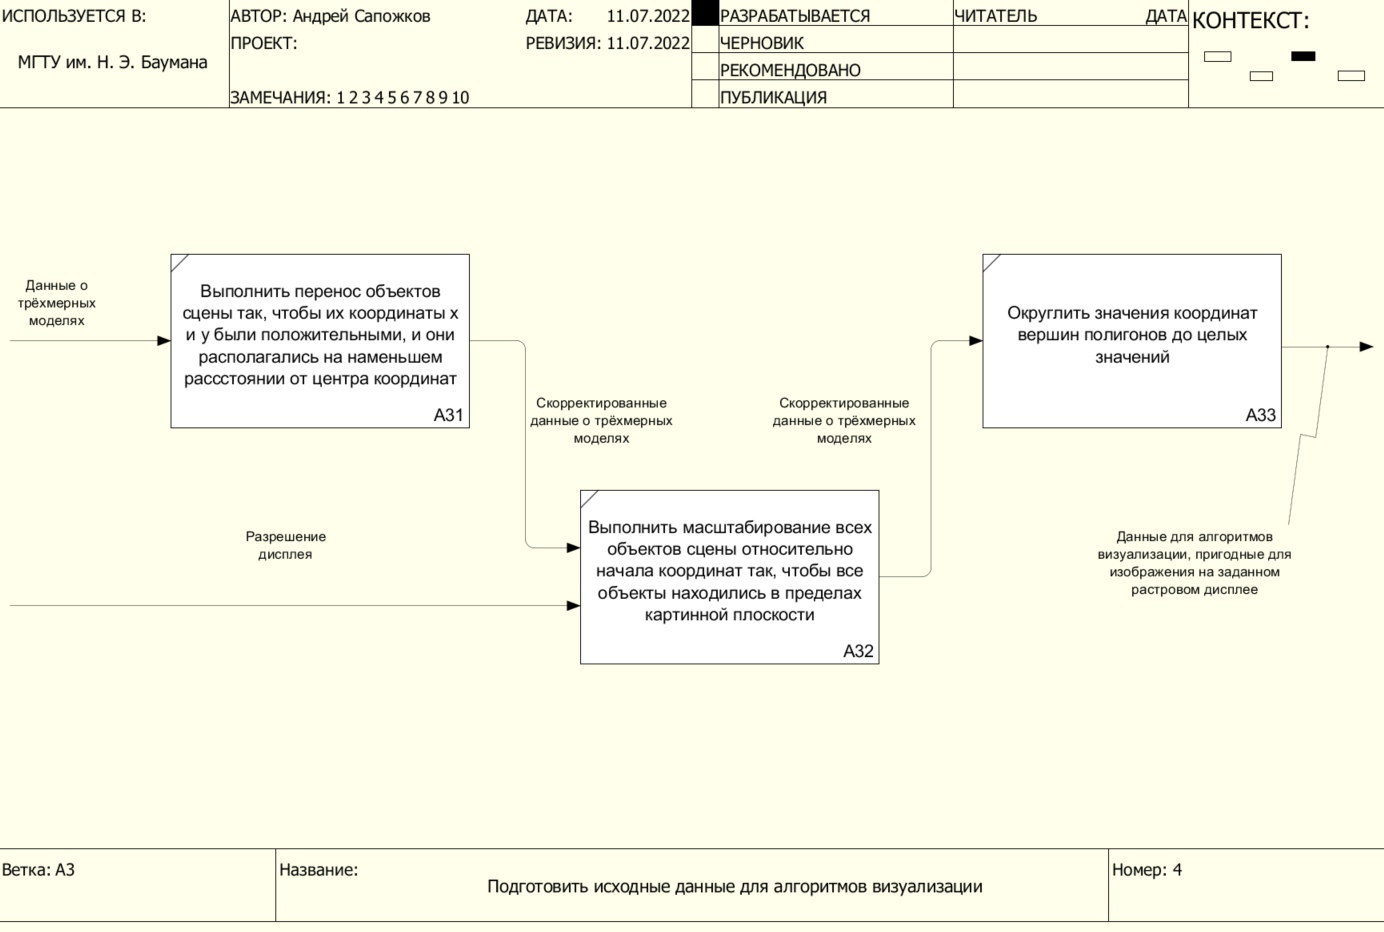
\includegraphics[width=\textwidth ]{img/IDEF0/A3_decomposition.jpg}
	\caption{Декомпозиция уровня A3.}
\end{figure} 

\begin{figure}[h]
	\centering
	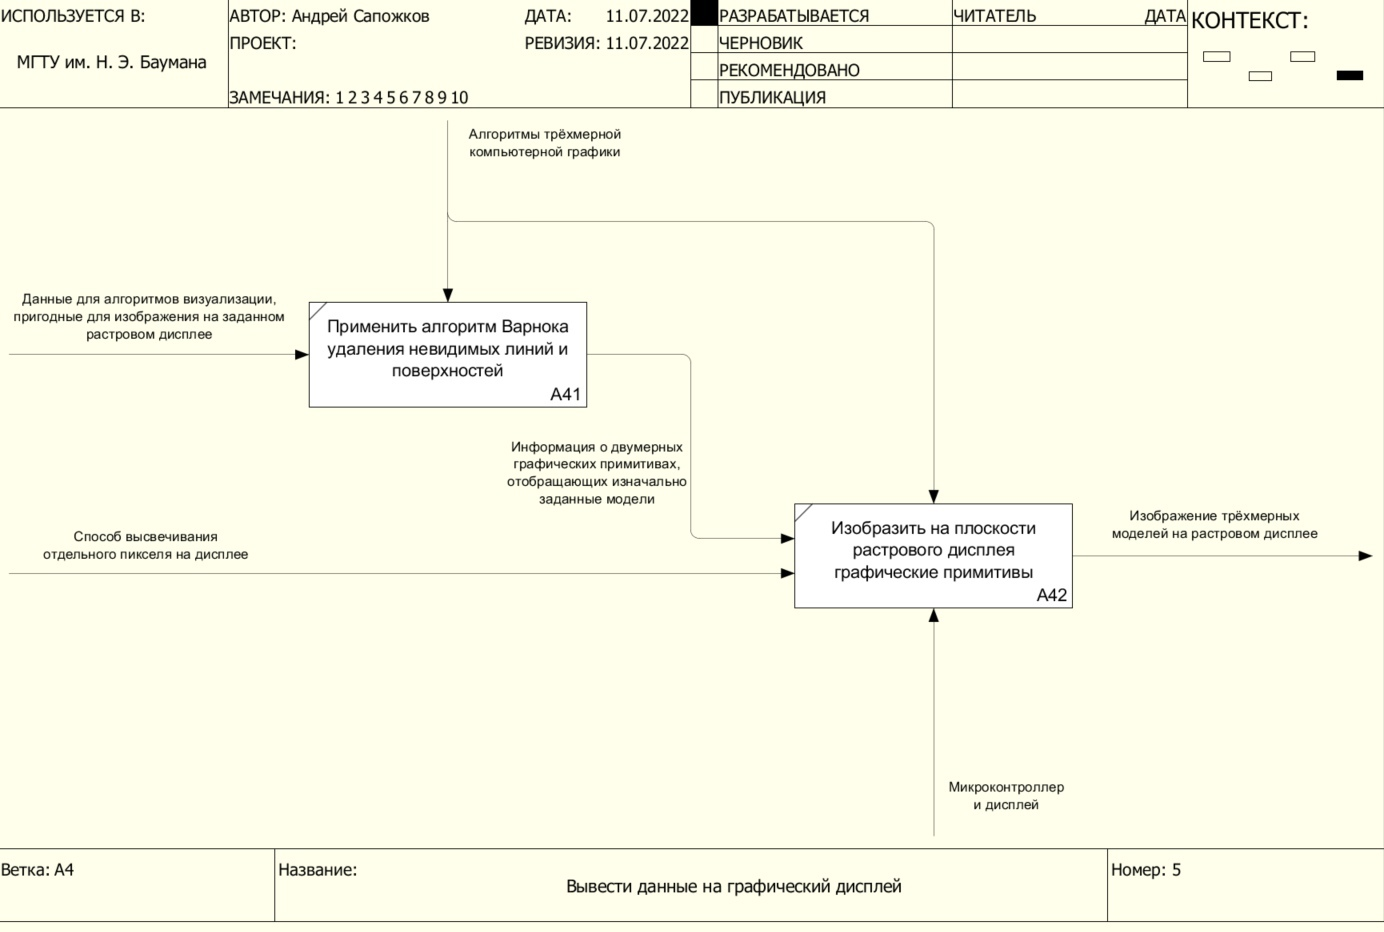
\includegraphics[width=\textwidth ]{img/IDEF0/A4_decomposition.jpg}
	\caption{Декомпозиция уровня A4.}
\end{figure} 

%%% Local Variables: 
%%% mode: latex
%%% TeX-master: "rpz"
%%% End: 
